\documentclass[preprint,12pt]{elsarticle}

\usepackage{amsmath,amssymb}
\usepackage{booktabs}
\usepackage{graphicx}
\usepackage{hyperref}
\usepackage{siunitx}
\setlength{\emergencystretch}{3em}

\journal{Astrodynamics}

\begin{document}

\begin{frontmatter}

\title{A Reproducible CR3BP Benchmark Resource for Low-Thrust Cislunar Missed-Thrust Initialization}

\author[aff1]{Anonymous Author}
\address[aff1]{Manuscript prepared for review; affiliation omitted in this draft}

\begin{abstract}
This paper presents a reproducible normalized Earth--Moon CR3BP benchmark resource for low-thrust cislunar missed-thrust initialization. The scope is preliminary algorithm benchmarking and provenance, not flight design, high-fidelity validation, SPICE/ephemeris propagation, production robust optimization, or operational targeting; all terminal-error thresholds are normalized screening tolerances. The resource archives source states, outage masks, configurations, result CSV/JSON files, generated tables and figures, cached force-model contrasts, and an artifact manifest. Under equal true trajectory-evaluation budgets, the initializer comparison does not support quantum or QAOA superiority: the configured statevector-QAOA initializer is weaker than the strongest classical initializers in the 30-seed main-method package, and optimized simulated QAOA is not statistically superior to surrogate-QUBO simulated annealing in the focused ablation. The positive evidence is narrower. A duty-cycle prior helps several samplers find refinable high-duty schedules, and the continuous-backend/provenance ladder separates selected-branch evidence, all-mask diagnostics, all-configured-mask rows, deterministic replay, and force-model stress. A new independent-midpoint Hermite--Simpson all-configured CR3BP headroom row optimizes all eight one-segment outage masks at phase time $0.4$ and $a_{\max}=0.2$, reaching nominal error $0.0111$ and all-configured worst error $0.0774$ while retaining a max-function-evaluation caveat. The hard-catalog tail-coast case is also normalized-CR3BP only: its all-configured one/two-segment row replays exactly from persisted accepted controls, but the same controls fail bicircular solar-tidal stress and fixed-phase bicircular retuning. The contribution is therefore an auditable benchmark resource with calibrated negative and positive evidence, not fuel optimality, certified robustness, production solver parity, or quantum advantage.
\end{abstract}

\begin{keyword}
Trajectory optimization benchmark \sep low-thrust trajectory optimization \sep cislunar dynamics \sep missed-thrust recovery \sep robust initialization \sep binary schedules \sep CR3BP \sep QUBO
\end{keyword}

\end{frontmatter}

\section{Introduction}

Electric low-thrust propulsion enables propellant-efficient cislunar transfers, but it also makes trajectory design highly sensitive to the initial guess supplied to a nonlinear optimizer. A practical design must determine both continuous thrust magnitudes and directions and a qualitative maneuver structure: which intervals thrust, coast, or recover after an interruption. For astrodynamics researchers, this creates a reproducibility problem as much as an algorithm problem. A proposed initializer is difficult to interpret unless the schedule objective, missed-thrust masks, continuous recovery backend, evaluation budget, and failure cases are all visible.

Missed-thrust robustness is a demanding test of that pipeline. Safe modes, propulsion interruptions, or operations-driven thrust outages can invalidate a nominal low-thrust transfer. Grebow and McCarty show that including missed-thrust branches in low-thrust cislunar design can greatly reduce recovery propellant for week-scale outages \cite{grebow2020missed}. Sinha and Beeson identify initial-guess generation as a bottleneck for low-thrust trajectory design with missed-thrust robustness \cite{sinha2025initial}. This paper therefore asks a benchmark question rather than a quantum-performance question:
\begin{quote}
Can a reproducible CR3BP benchmark resource reveal which missed-thrust initializers produce refinable schedules, which failure modes are caused by the continuous backend, and how surrogate-QUBO and simulated-QAOA initializers compare with strong classical samplers under equal trajectory-evaluation budgets?
\end{quote}

Binary and QUBO formulations are included because they are a natural way to encode thrust-window availability, and because recent low-thrust studies have explored binary/QUBO and quantum-assisted formulations \cite{degrossi2025transcription,moretta2026quantum}. They are not the headline claim. In this paper QUBO and QAOA are evaluated initializer families inside a broader robust-trajectory benchmark; the continuous trajectory remains a classical optimal-control problem, and negative evidence is reported as part of the contribution.

The paper makes four contributions for a trajectory-optimization audience.
First, it defines and archives a normalized Earth--Moon CR3BP benchmark resource with source states, missed-thrust masks, configurations, result artifacts, generated tables/figures, metadata, and a machine-readable manifest.
Second, it reports an equal-budget initializer comparison with a negative QAOA/sampler-superiority result: duty-cycle-aware schedules can be refinable, but the tested simulated QAOA variants do not dominate strong classical samplers or all-windows continuous refinement.
Third, it adds a continuous-backend and replay/provenance ladder that separates selected-branch evidence, all-mask diagnostics, all-configured-mask evidence, accepted-control replay, and recorded force-model stress.
Fourth, it records an external-validity boundary through cached Horizons force-model contrast, bicircular solar-tidal stress failures, and negative fixed-phase bicircular retuning of the hard-catalog tail-coast case.

The contribution is the schedule-initializer benchmark layer, not a replacement for production sequential-convex, collocation, or indirect low-thrust tools. Those mature solvers are downstream consumers and related-work comparators for a schedule or continuous-control initial guess. The controls used here--all-windows continuous refinement, direct shooting, compact collocation, continuation, and tail-coast diagnostics--are included to isolate whether the discrete schedule initializer adds value before handing the problem to stronger continuous machinery.

This framing is a natural fit for an astrodynamics methods journal even with negative quantum and robustness outcomes. The artifact is a cislunar trajectory-optimization resource: it exposes schedule-initializer failure modes, continuous-backend sensitivity, missed-thrust accounting, replay provenance, and force-model stress boundaries in a way that downstream astrodynamics solvers can use as controlled initialization tests. The value is therefore the audited benchmark and negative evidence, not a claim of a superior optimizer.

The claims are intentionally narrow. The experiments use normalized CR3BP dynamics, screening thresholds, configured outage families, and research-grade continuous backends. They do not establish quantum advantage, high-fidelity mission validation, fuel-optimal recovery, certified flight design, or universal missed-thrust robustness.

\section{Related Work}

\subsection{Low-thrust trajectory optimization}

Low-thrust trajectory optimization has a mature literature spanning indirect methods, direct transcription, collocation, global search, sequential convex programming, and hybrid approaches. Morante et al. survey low-thrust optimization as a hybrid optimal-control problem with both continuous and discrete structure \cite{morante2021survey}. In the Earth--Moon system, Ozimek and Howell computed low-thrust transfers to libration-point orbits and showed the role of CR3BP structure in preliminary design \cite{ozimek2010low}. Pritchett, Howell, and Grebow used collocation, trajectory stacking, orbit chaining, and continuation to compute low-thrust transfers in the restricted three-body problem, including NRHO-to-DRO examples \cite{pritchett2017collocation}. More recent cislunar and deep-space solvers include successive convex optimization for libration-point transfers \cite{kayama2022successive}, convex-programming approaches for rapid low-thrust trajectory design \cite{hofmann2021rapid}, thrust-regularized convex optimization \cite{morelli2024regularization}, indirect forward-backward shooting in complex dynamics \cite{sidhoum2024indirect}, and adaptive-mesh sequential convex programming \cite{kumagai2024adaptive}. These methods are mature trajectory-design baselines; the present work is not proposed as a replacement for them.

For preliminary cislunar design, the Circular Restricted Three-Body Problem is widely used because it captures the nonlinear Earth--Moon dynamical environment while keeping algorithmic studies tractable. The NASA/JPL Three-Body Periodic Orbits API provides normalized periodic-orbit states, periods, Jacobi constants, stability indices, and system constants for families such as halo orbits and distant retrograde orbits \cite{jplPeriodicOrbits}. The catalog-derived benchmark in this paper uses those states as transparent boundary-condition seeds. Its purpose is to expose initialization and recovery failure modes, not to certify an operational transfer.

\subsection{Robust and missed-thrust trajectory design}

Missed-thrust design has been studied through margin analysis, expected-thrust formulations, virtual recovery trajectories, robust optimal control, and branching trajectory methods. Rubinsztejn et al. embed expected thrust fraction into deterministic trajectory design and report improved resilience to missed-thrust scenarios \cite{rubinsztejn2021expected}. Venigalla et al. formulate multi-objective low-thrust trajectory optimization with missed-thrust recovery margin \cite{venigalla2022multi}. Grebow and McCarty specifically study low-thrust cislunar transfers, including NRHO-to-DRO transfers, and optimize branching trajectories for outage recovery \cite{grebow2020missed}. Sinha and Beeson focus on initial-guess generation for robust low-thrust missed-thrust design and compare conditional and nonconditional global-search strategies \cite{sinha2025initial}. Robust cislunar low-thrust optimization has also advanced through sequential convex programming and covariance steering; Kumagai and Oguri use chance-constrained covariance steering to design nominal trajectories and correction policies under uncertainty in the Earth--Moon CR3BP \cite{kumagai2025robust}. Broader uncertainty-aware low-thrust design includes nonlinear programming and forward-backward shooting under uncertainty \cite{varghese2026uncertainty}, and missed-thrust robustness has recently been addressed with sequential convex programming \cite{sekine2026missedscp}. State-dependent trust-region ideas for autonomous spacecraft SCP further illustrate the level of numerical machinery expected in robust flight-dynamics workflows \cite{bernardini2024trust}. These works set a high bar for any initializer: a useful discrete schedule must ultimately feed a continuous optimizer that can produce robust feasible trajectories.

\subsection{QUBO/QAOA initializers}

Quantum annealers and QAOA target discrete optimization models such as Ising Hamiltonians and QUBOs. A QUBO minimizes
\begin{equation}
E(x) = c + \sum_i a_i x_i + \sum_{i<j} b_{ij} x_i x_j,\qquad x_i\in\{0,1\},
\end{equation}
which is convertible to the Ising form used in quantum annealing and many gate-model workflows \cite{dwaveQubo,glover2018qubo}. Farhi et al. introduced QAOA as a gate-model variational algorithm for approximate combinatorial optimization \cite{farhi2014qaoa}. Shukla and Vedula formulated trajectory optimization as a discrete search problem and argued that quantum search can provide speedups for suitably discretized cases \cite{shukla2019trajectory}. De Grossi et al. provide the closest low-thrust QUBO precedent \cite{degrossi2025transcription}. This paper uses QUBO and QAOA only for the discrete initialization layer; the continuous trajectory remains a classical optimal-control problem.

\subsection{Benchmark gap}

The targeted catalog benchmark in this paper is deliberately harder than the teacher-controlled case because cislunar transfers between stable or nearly stable periodic orbits are known to be sensitive to the continuous initial guess. The gap addressed here is therefore diagnostic rather than algorithmic replacement: the paper asks how binary schedule samplers, including QUBO/QAOA variants, behave under equal trajectory-evaluation budgets when missed-thrust penalties are included and when their schedules are handed to research-grade continuous recovery backends. Existing missed-thrust and robust cislunar studies optimize trajectories, recovery branches, correction policies, or mission-design workflows. This paper instead packages reusable source states, masks, configurations, recorded controls, and evidence semantics so those stronger trajectory-design tools can be compared against a transparent initialization benchmark. Production SCP, collocation, and indirect tools remain the appropriate downstream solvers for mission-quality design. The all-windows continuous row and the continuous-backend diagnostics are the relevant controls for this benchmark layer because they test whether schedule selection improves the initial condition passed downstream. The resulting artifact package complements production-oriented studies by making failure modes, claim boundaries, and reproducibility provenance explicit.

\section{Problem Formulation}

\subsection{Forced CR3BP dynamics}

The spacecraft state is
\begin{equation}
s = [x,y,z,\dot{x},\dot{y},\dot{z}]^\top
\end{equation}
in the normalized Earth--Moon rotating frame. With mass parameter $\mu$, distances to the primary and secondary bodies are
\begin{align}
r_1 &= \sqrt{(x+\mu)^2+y^2+z^2},\\
r_2 &= \sqrt{(x-1+\mu)^2+y^2+z^2}.
\end{align}
The forced CR3BP equations are
\begin{align}
\ddot{x} &= 2\dot{y}+x-\frac{(1-\mu)(x+\mu)}{r_1^3}-\frac{\mu(x-1+\mu)}{r_2^3}+a_x,\\
\ddot{y} &= -2\dot{x}+y-\frac{(1-\mu)y}{r_1^3}-\frac{\mu y}{r_2^3}+a_y,\\
\ddot{z} &= -\frac{(1-\mu)z}{r_1^3}-\frac{\mu z}{r_2^3}+a_z.
\end{align}

The transfer duration $T$ is divided into $N$ uniform segments. A binary variable $x_i\in\{0,1\}$ gates thrust availability during segment $i$. During the discrete search stage, a deterministic target-seeking steering law maps the binary schedule to a propagated trajectory,
\begin{equation}
g(s) = K_r(r_f-r) + K_v(v_f-v),\qquad
a_i(s) = x_i a_{\max}\frac{g(s)}{\|g(s)\|+\epsilon}.
\end{equation}
This steering law is not claimed to be optimal. It creates a repeatable map from a bitstring to a trajectory so that discrete schedules can be ranked before continuous refinement. A separate oracle diagnostic, introduced only for the teacher-controlled benchmark, initializes refinement from the hidden continuous controls used to generate the target. That diagnostic is not a competing initializer; it tests whether the refinement formulation can recover the known feasible trajectory when continuous-control initialization is no longer the bottleneck.

\subsection{Missed-thrust masks and robust binary cost}

Let $\mathcal{M}$ denote a set of outage masks. Each mask zeros thrust in a one- or two-segment contiguous window. For a nominal schedule $x$, the outage-realized schedule is $x\odot m$. The scaled terminal error under mask $m$ is
\begin{equation}
e_m(x)=
\left\|\begin{bmatrix}
(r_T(x\odot m)-r_f)/\ell_r\\
(v_T(x\odot m)-v_f)/\ell_v
\end{bmatrix}\right\|_2.
\end{equation}

The trajectory-evaluated robust binary objective is
\begin{align}
J(x) = &\; w_n e_0(x) + w_w \max_{m\in\mathcal{M}} e_m(x)
+ w_d\left(\max_{m\in\mathcal{M}} e_m(x)-e_0(x)\right) \nonumber\\
&+ w_p\frac{1}{N}\sum_{i=1}^{N}x_i
+ w_s\frac{1}{N-1}\sum_{i=1}^{N-1}|x_{i+1}-x_i|.
\end{align}
The terms penalize nominal miss distance, worst outage miss distance, missed-thrust degradation, active thrust fraction, and thrust/coast switching.

\section{Initializer Families}

\subsection{QUBO surrogate}

Because $J(x)$ depends on nonlinear propagation and outage evaluation, it is not itself a QUBO. The method therefore fits
\begin{equation}
\widehat{J}(x)=c+\sum_i a_i x_i+\sum_{i<j}b_{ij}x_i x_j
\end{equation}
from trajectory-evaluated samples $\{x^{(k)},J(x^{(k)})\}_{k=1}^{K}$ using ridge-regularized least squares:
\begin{equation}
\min_{\theta}\sum_{k=1}^{K}\left(J(x^{(k)})-\widehat{J}(x^{(k)};\theta)\right)^2
+\lambda\|\theta\|_2^2.
\end{equation}
The fitted QUBO is then sampled by classical QUBO simulated annealing or converted to a diagonal cost Hamiltonian for statevector QAOA. The present experiments use QAOA only as a small simulated gate-model sampler; no hardware quantum advantage is implied.

\subsection{Discrete initializers}

The experiments compare random search, cross-entropy search, a genetic algorithm, true-objective simulated annealing, surrogate QUBO simulated annealing, and statevector QAOA. Random search and true-objective simulated annealing evaluate propagated schedules directly. Cross-entropy updates Bernoulli segment probabilities from elite samples. The genetic algorithm uses elitism, crossover, and mutation. The QUBO and QAOA methods use true trajectory evaluations to train $\widehat{J}$, then validate their best sampled schedules with the true objective.

Budget accounting is therefore reported in two ways: solver true evaluations exclude shared QUBO training, while total true evaluations include QUBO training. Equal total-evaluation comparisons are the relevant fair comparison.

\subsection{Continuous branch-recovery refinement}

The refinement stage converts a selected binary schedule into a continuous low-thrust candidate by optimizing piecewise-constant acceleration vectors only in active windows. Refined accelerations are projected to the Euclidean thrust ball $\|u_i\|_2\leq a_{\max}$ before propagation and persistence. The branch-recovery mode optimizes a nominal control sequence plus selected-outage-specific post-outage recovery controls. Its least-squares residual includes nominal terminal error, selected outage terminal error, fuel regularization, control regularization, and inter-segment smoothness. A run is counted as successful only if both the nominal terminal error and the selected missed-thrust worst error are below the configured thresholds.

The paper also reports an all-mask diagnostic: after refinement on selected outages, every one- and two-segment outage mask is evaluated without claiming that all masks were optimized. This separates selected-branch recovery success from universal outage robustness.

\section{Experimental Setup}

\subsection{Common dynamics and source state}

All experiments use normalized Earth--Moon CR3BP dynamics with $\mu=0.01215058560962404$. The common initial state is taken from the first row of an Earth--Moon L2 southern halo query with period in $[1.55,1.65]$ TU from the NASA/JPL periodic-orbit API:
\begin{equation}
s_0=[1.0324985738,0,-0.1884844917,0,-0.1249781287,0].
\end{equation}
This state is NRHO-like in the sense that it lies in the L2 southern halo family, but the paper treats it as a normalized benchmark state, not a certified operational NRHO.

\subsection{Dimensional scale and threshold interpretation}
\label{sec:dimensional-scale}

The normalized Earth--Moon scale is used only to interpret orders of magnitude. Taking the public NASA average Earth--Moon distance as $1$ LU $\approx 384{,}400$ km \cite{nasaSpacePlaceMoonDistance}, the recorded CR3BP normalization gives $1$ TU $\approx 375{,}190.259$ s $=4.34248$ days, velocity unit $\approx 1.02455$ km/s, and acceleration unit $\approx 2.73074$ mm/s$^2$. Thus the main phase-shift transfer time $T=0.5$ TU is about $2.17$ days, while the hard-catalog tail-coast recovery case with $T=4.0$ TU is about $17.37$ days. The acceleration bounds used in the phase-shift and high-thrust diagnostics correspond to $a_{\max}=0.2\approx 0.546$ mm/s$^2$ and $a_{\max}=1.0\approx 2.731$ mm/s$^2$, respectively.

The terminal-error thresholds are screening tolerances in the normalized metric
\begin{equation}
\sqrt{\|\Delta r\|_2^2+\|\Delta v\|_2^2/0.35^2},
\end{equation}
not flight navigation or operational targeting tolerances. If velocity error is zero, the nominal threshold $0.09$ corresponds to a position-only error of about $34{,}596$ km, and the selected-recovery threshold $0.17$ corresponds to about $65{,}348$ km. If position error is zero, the same thresholds correspond to velocity-only errors of about $32.3$ m/s and $61.0$ m/s under the configured velocity scale. This scale is the reason the manuscript frames the results as preliminary design and initializer benchmarking rather than operational targeting.

\subsection{Benchmark families}

Two benchmark families define the main evidence path. The harder catalog-derived family uses a distant retrograde orbit seed from an Earth--Moon DRO query,
\begin{equation}
s_{\mathrm{DRO}}=[0.8161260827,0,0,0,0.5076556931,0],
\end{equation}
and generates the target by ballistic propagation of that seed. The original catalog-derived schedule run uses $T=2.7$ TU, $N=12$, $a_{\max}=0.055$, and one- and two-segment outage masks. It remains negative evidence in the supplement. The main hard-catalog result instead reports a later locked-nominal tail-coast continuous-backend diagnostic at $T=4.0$ TU, $N=14$, and $a_{\max}=1.0$, where the final five nominal control segments are constrained to zero and all configured one- and two-segment masks are selected and evaluated in one fixed-final-time row.

The non-teacher phase-shift family is derived from the same JPL L2 southern halo source state $s_0$. The target is generated by zero-thrust CR3BP propagation of $s_0$ for a phase time of $0.3$ TU, while the transfer must arrive at that target after $T=0.5$ TU. A zero-thrust trajectory has normalized terminal error $0.3758$, so the case is not a do-nothing pass. The primary initializer benchmark uses $N=12$, $a_{\max}=0.2$, one-segment outage masks, and a duty-cycle prior
\begin{equation}
J_{\rho}(x)=w_{\rho}\left(\frac{1}{N}\sum_{i=1}^{N}x_i-\rho\right)^2,
\end{equation}
with $\rho=11/12$ and $w_{\rho}=12$. This prior is not an oracle trajectory correction; it encodes a preference for one coast window while preserving a dense low-thrust arc.

The supplement preserves the secondary diagnostic families: the catalog pilot and QUBO fit diagnostics, feasibility and direct multiple-shooting stress tests, locked-nominal and delayed-arrival hard-catalog recovery packages, bounded phase-suite and robust-margin rows, direct-collocation and Hermite--Simpson baselines, dense-repair and legacy cardinality ablations, and the teacher-controlled feasible benchmark. These diagnostics explain provenance and failure modes but are not promoted to headline evidence in the main article.

\subsection{Metrics}

The primary metrics are refined nominal terminal error, refined selected missed-thrust worst error, all-mask diagnostic worst error, schedule active fraction, nominal and recovery fuel, total true trajectory evaluations, and refinement success rate. A run is counted as a robust refinement success only when both the nominal terminal error and the selected missed-thrust worst error are below the configured thresholds. Unless otherwise stated, those thresholds are $0.09$ for nominal success and $0.17$ for selected robust recovery success.

The main $N=12$ duty-cycle-prior statistics package repeats seven methods over 30 deterministic seeds, for 210 raw method--seed rows, and reports Wilson success intervals, paired per-seed success differences, bootstrap confidence intervals for mean selected-worst-error differences, and exact two-sided sign tests. A separate focused QAOA-depth package repeats the QUBO-derived methods over 30 deterministic seeds, for 150 raw method--seed rows. The hard-catalog tail-coast row \texttt{tail\_coast\_all\_one\_two\_segment\_t5\_portfolio} uses the same thresholds, selects all configured one- and two-segment masks in one case row, and reports optimizer convergence separately from threshold feasibility so late-tail direct evaluations without recovery variables are not mistaken for optimizer-converged branch solves.

\section{Results}

The main results are screening evidence for a normalized CR3BP benchmark. The dimensional caveat in Section~\ref{sec:dimensional-scale} applies to every table: the $0.09/0.17$ thresholds correspond to large position-only or velocity-only errors and should not be read as operational targeting tolerances. Secondary tables and figures are retained in the supplement so that the main article follows the primary claim path, while the evidence-synthesis table below cross-indexes representative rows from those recorded artifacts.

\subsection{Claim hierarchy}

Table~\ref{tab:claim_evidence_hierarchy} records the claim boundary used throughout the paper. It lists each headline claim, its primary artifacts, its status, and interpretations that are explicitly prohibited by the evidence.

\begin{table}[t]
\centering
\caption{Compact claim hierarchy for the manuscript. Pass/fail labels refer only to the configured normalized screening evidence, not to flight validation.}
\label{tab:claim_evidence_hierarchy}
{\renewcommand{\arraystretch}{0.75}
\resizebox{0.95\textwidth}{!}{
\begin{tabular}{p{0.20\textwidth}p{0.32\textwidth}p{0.19\textwidth}p{0.29\textwidth}}
\toprule
Claim & Primary artifacts & Status & Prohibited interpretations \\
\midrule
Benchmark resource & Source states, configs, result CSV/JSON, generated tables/figures, cache metadata, and artifact manifest & Pass as an auditable normalized CR3BP resource & Operational targeting, flight certification, or mission-design completeness \\
Initializer comparison & 30-seed raw results, success intervals, paired comparisons, threshold sensitivity, and QAOA/QUBO ablation tables & Negative for quantum/QAOA superiority; positive only for duty-cycle-aware refinability & Quantum advantage, hardware evidence, or sampled-method dominance over all-windows continuous refinement \\
Continuous-backend diagnostics & Continuation, direct collocation, Hermite--Simpson, replay/stress sidecars, and metadata packages & Mixed: several scoped CR3BP rows pass configured screens, while harder rows fail & Certified solver parity, fuel optimality, or universal missed-thrust robustness \\
Hard-catalog tail-coast & Tail-coast recovery CSV, accepted-control replay CSV/metadata, branch audit, and threshold audit & Scoped pass under normalized CR3BP for all 27 configured one/two masks & High-fidelity robustness, broader outage-family robustness, production solver parity, or quantum evidence \\
Force-model stress bridges & Cached Horizons contrast, bicircular solar-tidal stress CSV/metadata, and generated tables & Contrast-only for Horizons; negative threshold outcome for bicircular replay & SPICE validation, ephemeris flight validation, accepted-control high-fidelity replay, or DOI/release proof \\
\bottomrule
\end{tabular}}}
\end{table}

\subsection{Claim-ledger summary}

The generated claim ledger in \path{data/results/claim_evidence_ledger/} is retained as a reviewer-facing audit artifact rather than as a dense main-text table. It reads recorded CSV/JSON files only and separates selected-branch evidence, all-mask diagnostics, all-configured-mask rows, accepted-control replay, force-model contrast, stress probes, and retuned-recovery evidence. The full ledger, tail-coast threshold audit, and tail-coast branch audit are reported in the supplement. The main text keeps the compact hierarchy in Table~\ref{tab:claim_evidence_hierarchy} and the cross-backend synthesis in Table~\ref{tab:evidence_synthesis}; together they state the operative boundaries without turning the article into an artifact listing.

For practitioners, the reporting lesson is concrete: include the all-windows continuous control, do not collapse selected-branch and all-mask semantics, preserve negative QAOA/QUBO evidence, and archive provenance in machine-readable artifacts. In the current ledger, the new independent-midpoint Hermite--Simpson headroom row is all-configured one-segment normalized-CR3BP evidence, while the earlier independent-HS p=0.4 row remains selected-branch/all-mask diagnostic evidence.

\subsection{Cross-backend evidence synthesis}

Table~\ref{tab:evidence_synthesis} is generated by \path{scripts/run_evidence_synthesis.py}. The script reads only recorded CSV/JSON artifacts and writes \path{data/results/evidence_synthesis/evidence_synthesis.csv}, \path{data/results/evidence_synthesis/evidence_synthesis_metadata.json}, and the LaTeX table used here. It is not a new optimization run. Its purpose is to put the broader validation axes into the main claim path without overstating them.

The synthesis clarifies the positive contribution. The 30-seed threshold-sensitivity row shows that at the tight $(0.050,0.090)$ check every sampled method is $0/30$ while all-windows continuous remains $30/30$, so the paper does not claim sampler superiority. The continuation-extension rows show that all-mask direct multiple-shooting continuation can meet a tighter $(0.065,0.100)$ phase-shift screen for all one-segment masks and for all configured one/two masks, but not the $0.05$ nominal headroom check. The direct-collocation and earlier independent-midpoint Hermite--Simpson rows show compact continuous backends with tight selected/all diagnostics while preserving selected-branch semantics. The new independent-midpoint Hermite--Simpson headroom package upgrades that phase-shift evidence to an all-configured one-segment row at phase time $0.4$ and $a_{\max}=0.2$: all eight configured masks are selected and evaluated, with nominal error $0.0111$ and selected/all worst error $0.0774$. The hard-catalog rows show that the fixed-final-time pass is scoped to the tail-coast locked-nominal backend; an independent-HS selected-outage hard-catalog diagnostic remains a negative result.

\begin{table}[t]
\centering
\caption{Cross-backend evidence synthesis generated from recorded artifacts only. Error entries are nominal / selected-worst / all-mask-worst in the normalized terminal metric. Tighter pass statuses use all-mask diagnostics conservatively; selected-branch rows remain diagnostics unless all configured masks are explicitly selected.}
\label{tab:evidence_synthesis}
\resizebox{\textwidth}{!}{\begin{tabular}{llllllll}
\toprule
Axis & Representative evidence & Role & Scope & Nom / Sel / All & Configured & Tighter or near-tight status & Practitioner lesson \\
\midrule
30-seed threshold sensitivity & tight (0.050,0.090) pass counts & sampled binary initializers versus all-windows continuous & 30 deterministic seeds; selected one-segment recovery masks & counts only & see source threshold table & sampled methods 0/30; all-windows 30/30 & Tight screening exposes margin limits of sampled high-duty schedules; the positive result is the benchmark diagnostic, not sampler superiority. \\
continuation-extension multiple shooting & all\_single\_p04\_warm\_from\_p03 & all one-segment continuous continuation from p=0.3 & 8/8 configured one-segment masks selected and evaluated & 0.0531 / 0.0139 / 0.0139 & True & 0.065/0.10: True; 0.05/0.09: False & All-mask continuation has headroom at p=0.4 under 0.065/0.10 screening, but the nominal error is above 0.05. \\
continuation-extension multiple shooting & two\_segment\_n8\_p03\_cold & cold all one/two-mask continuous continuation & 15/15 configured one- and two-segment masks selected and evaluated & 0.0612 / 0.0435 / 0.0435 & True & 0.065/0.10: True; 0.05/0.09: False & A broader one/two-mask phase-shift row passes 0.065/0.10 all-mask diagnostics, but not the 0.05 nominal headroom check. \\
direct-collocation baseline & selected-branch p=0.4 & compact trapezoidal selected-branch collocation & 1 selected outage branch; 12 one-segment all-mask diagnostics & 0.0357 / 0.0191 / 0.0602 & True & 0.065/0.10: True; 0.05/0.09: True & Compact collocation can be tight on this selected branch, but unselected masks remain diagnostics and should be reported. \\
independent-midpoint Hermite-Simpson & ihs\_phase\_p04\_amax02\_warm\_from\_p03 & selected-branch independent-midpoint collocation with tighter thrust & 3 selected outage branches; 8 one-segment all-mask diagnostics & 0.0197 / 0.0188 / 0.0532 & True & 0.065/0.10: True; 0.05/0.09: True & Independent midpoint controls meet tight all-mask diagnostics on this phase-shift row even at amax=0.2. \\
hard-catalog tail-coast recovery & tail\_coast\_all\_one\_two\_segment\_t5\_portfolio & locked-nominal fixed-final-time tail-coast branch portfolio & 27/27 configured one- and two-segment masks selected and evaluated & 0.0230 / 0.0936 / 0.0936 & True & 0.05/0.10: True; 0.05/0.09: False & The hard-catalog pass is real but scoped to the tail-coast backend; it passes 0.05/0.10 and narrowly misses 0.05/0.09 because the selected/all worst error is 0.0936063931709301. \\
independent-midpoint Hermite-Simpson & ihs\_catalog\_dro\_tf4\_amax1\_selected1 & bounded selected-outage independent-midpoint collocation negative diagnostic & 1 selected outage branch; 15 one/two-mask all-mask diagnostics & 4.2644 / 11.0843 / 11.0843 & False & 0.065/0.10: False; 0.05/0.09: False & The hard-catalog result is not a generic continuous-backend pass; this independent-HS selected-outage diagnostic fails badly. \\
\bottomrule
\end{tabular}
}
\end{table}

\subsection{Tail-coast hard-catalog diagnostic}

Table~\ref{tab:tail_coast_recovery} reports the strongest hard-catalog fixed-final-time result. The setup solves and freezes a locked nominal control, then refines it with the final five nominal control segments constrained to exact zero. Branches keep the original target and original final time; no delayed target or added recovery horizon is used. The nominal-only provenance row has tail-coast nominal error $0.022992$ and therefore passes the nominal screening threshold, while its masked-nominal all-mask diagnostic remains $27.8351$ because no branch recovery is run.

The headline row is \texttt{tail\_coast\_all\_one\_two\_segment\_t5\_portfolio}. It sets \texttt{outage\_lengths=[1,2]}, selects all configured masks, and evaluates all 27 selected masks in one fixed-final-time case row. The row reaches tail-coast nominal error $0.02299233817855882$, selected fixed-time worst error $0.0936063931709301$, and all-mask fixed-time diagnostic worst error $0.0936063931709301$, so it meets the configured $0.09/0.17$ screening thresholds. The branch portfolio evaluates deterministic fallback starts for four branches, charges $5929$ function evaluations, and records runtime about $1833.6$ s in the current CSV. Among branches with post-outage recovery variables, the optimizer-converged count is $25/25$. The remaining two late-tail masks have no post-outage recovery variables; they are direct fixed-final-time threshold evaluations rather than optimizer-converged branch solves. Therefore \texttt{branch\_optimizer\_all\_success=false} remains a conservative CSV accounting flag even though \texttt{meets\_thresholds=true}.

This result is deliberately scoped. It is fixed-final-time continuous-backend evidence with a locked nominal control, final-five-segment coast, configured one- and two-segment masks, fallback starts, and late-tail no-recovery-variable accounting. It is not a binary-sampler result, not QUBO/QAOA evidence, not fuel optimality, not high-fidelity validation, and not robustness to outage families beyond the configured masks.

\begin{table}[t]
\centering
\caption{Fixed-final-time tail-coast locked-nominal hard-catalog recovery. The combined row selects/evaluates all 27 configured one- and two-segment masks in one fixed-final-time case row; separate all-single and all-two-segment rows are retained as provenance/scope rows. Branches with post-outage recovery variables are optimized. No-recovery-variable late-tail branches are direct threshold evaluations, so false branch optimizer all-success flags are accounting caveats rather than threshold failures.}
\label{tab:tail_coast_recovery}
\resizebox{\textwidth}{!}{\begin{tabular}{llllllllllllllllllll}
\toprule
Case & Policy & Selected masks & Tail coast segments & Branch portfolio & Branch variants & Fallback starts & Accepted fallback by branch & Seed nominal error & Tail-coast nominal error & Selected fixed-time worst error & All-mask fixed-time diagnostic worst & Tail max |u| & Max ||u|| & Bound violation & nfev & Runtime (s) & Meets thresholds & Branch optimizer ran & Accepted branch optimizers converged \\
\midrule
tail\_coast\_all\_single\_t5\_portfolio & all\_single & 14 & 5 & True & ["regularized\_001", "terminal\_only"] & ["constant\_y\_plus\_0p5", "constant\_y\_minus\_0p5"] & [false, false, false, false, false, false, false, true, false, false, false, false, false, false] & 0.0131 & 0.0230 & 0.0230 & 0.0230 & 0.0000 & 1.0000 & 0.0000 & 2057 & 1145.7074 & True & True & False \\
tail\_coast\_nominal\_only\_t5 & 0 & 0 & 5 & False & ["configured"] & [] & [] & 0.0131 & 0.0230 & 0.0230 & 27.8351 & 0.0000 & 1.0000 & 0.0000 & 287 & 158.4524 & True & False & False \\
\bottomrule
\end{tabular}
}
\end{table}

\subsection{Replay and external-validity boundary}

The full accepted-control replay, nominal sidecar replay/stress, Horizons contrast, bicircular stress, and bicircular retuning tables are moved to the supplement. The main facts are concise. The focused accepted-control replay for \texttt{tail\_coast\_all\_one\_two\_segment\_t5\_portfolio} contains one nominal row and 27 branch rows; repropagation under the configured normalized CR3BP model gives zero nominal, branch, and maximum terminal-error delta at tolerance $10^{-10}$. That is deterministic replay of persisted controls, not a new solve or production solver parity.

The external-validity checks are deliberately negative. A cached JPL Horizons contrast for the same hard-catalog window samples 15 transfer nodes from a fixed 2026-Jan-01 TDB epoch and records Earth--Moon distance/rate variation, Sun distance/phase differences, and solar-tidal acceleration differences; it is a force-model contrast only, not SPICE validation or ephemeris propagation. Replaying the accepted controls with a simple bicircular solar-tidal term fails the configured thresholds: every nominal solar-tidal phase fails the $0.09$ nominal threshold, only $22/108$ branch-phase rows pass the $0.17$ branch threshold, and the maximum solar-tidal terminal error is $37.7596$. A fixed-phase retuning batch under the same simple bicircular model also remains negative: retuned nominal error is $0.316772$, configured branch pass count is $19/27$, maximum retuned branch error is $6.0299$, and strict branch pass count is $16/27$. The hard-catalog tail-coast pass is therefore foregrounded as normalized-CR3BP evidence only.

\subsection{Thirty-seed main-method statistics}

Tables~\ref{tab:phase_shift_cardinality_30seed} and~\ref{tab:phase_shift_cardinality_30seed_statistics}, together with Figure~\ref{fig:phase_shift_cardinality_30seed}, repeat the configured $N=12$ duty-cycle-prior method comparison over 30 deterministic seeds. The raw package contains 210 rows, i.e., 30 seeds times seven methods: random search, cross-entropy search, genetic search, true-objective simulated annealing, surrogate-QUBO simulated annealing, the configured statevector QAOA sampler, and all-windows continuous refinement.

The success-rate evidence strengthens the 10-seed result but does not create a quantum-performance claim. Random search succeeds in $11/30$ seeds, with Wilson 95\% interval $[0.219,0.545]$. Cross-entropy, genetic search, true-objective simulated annealing, surrogate-QUBO simulated annealing, and all-windows continuous refinement each succeed in $30/30$ seeds, with Wilson interval $[0.886,1.000]$. The configured \texttt{qaoa\_statevector} method succeeds in $13/30$ seeds, with interval $[0.274,0.608]$.

The paired error comparisons are more important for the aerospace interpretation. Against all-windows continuous refinement, every sampled method has a positive mean selected-worst-error difference; negative would favor the sampled method. The exact two-sided sign-test value is approximately $1.86\times10^{-9}$ for each sampler versus all-windows continuous refinement. Thus, the all-windows continuous baseline is not just equally successful for the strongest methods; it also gives lower selected-worst error on this benchmark. Against surrogate-QUBO simulated annealing, cross-entropy, genetic search, and true-objective simulated annealing tie the success rate and have small nonsignificant selected-worst-error deltas. Random search is worse. The configured statevector QAOA row has lower success and a positive mean selected-worst-error delta of $0.0153$ versus surrogate-QUBO simulated annealing, with exact sign-test $p=0.1849$.

This package therefore strengthens the statistics beyond a QAOA-only ablation while preserving the conservative conclusion. Duty-cycle priors help several samplers find feasible high-duty schedules, but all-windows continuous fuel regularization remains a stronger mechanism for selected-worst error in this benchmark, and the evidence does not support quantum advantage or QAOA superiority.

Table~\ref{tab:phase_shift_cardinality_30seed_thresholds} adds a threshold-sensitivity sanity check computed only from \path{data/results/phase_shift_cardinality_30seed/raw_results.csv}. At the stricter $(0.075,0.120)$ nominal/selected-worst thresholds, cross-entropy, genetic search, true-objective simulated annealing, surrogate-QUBO simulated annealing, and all-windows continuous refinement still pass $30/30$ seeds, while random search falls to $4/30$ and \texttt{qaoa\_statevector} remains $13/30$. At $(0.065,0.100)$ the sampled high-duty schedules largely stop passing, but all-windows continuous remains $30/30$. At the tight $(0.050,0.090)$ check, every sampled method is $0/30$ while all-windows continuous is still $30/30$. Thus stricter thresholds do not rescue sampled-method superiority; they quantify the margin limitation of the sampled schedules and reinforce the all-windows continuous lower-error diagnostic.

\begin{table}[t]
\centering
\caption{Thirty-seed $N=12$ duty-cycle-prior phase-shift method comparison. Values summarize 210 method--seed rows. QUBO/QAOA totals include 96 shared QUBO-training evaluations and 24 post-QUBO true candidate evaluations.}
\label{tab:phase_shift_cardinality_30seed}
\resizebox{\textwidth}{!}{\begin{tabular}{llllllllrrrrrrrrrrr}
\toprule
Benchmark & Method & Schedule repair & Refined schedule source & Comparison group & Solver best schedule & Refine candidate schedule & Refined schedule & Refined nominal error & Selected recovery worst error & All-mask diagnostic worst error & Solver best active fraction & Active target penalty & Refine candidate active fraction & Refined active fraction & Solver true evals & Shared QUBO train evals & Total true evals & Refine success \\
\midrule
catalog\_halo\_phase\_shift & random & identity & original solver candidate schedule & method\_comparison & mixed & mixed & mixed & 0.0928 & 0.1188 & 0.1277 & 0.8333 & 0.0833 & 0.8333 & 0.8333 & 120.0000 & 0.0000 & 120.0000 & 0.3667 \\
catalog\_halo\_phase\_shift & cross\_entropy & identity & original solver candidate schedule & method\_comparison & mixed & mixed & mixed & 0.0690 & 0.0941 & 0.1018 & 0.9167 & 0.0000 & 0.9167 & 0.9167 & 120.0000 & 0.0000 & 120.0000 & 1.0000 \\
catalog\_halo\_phase\_shift & genetic & identity & original solver candidate schedule & method\_comparison & mixed & mixed & mixed & 0.0675 & 0.0926 & 0.1018 & 0.9167 & 0.0000 & 0.9167 & 0.9167 & 120.0000 & 0.0000 & 120.0000 & 1.0000 \\
catalog\_halo\_phase\_shift & true\_sa & identity & original solver candidate schedule & method\_comparison & mixed & mixed & mixed & 0.0690 & 0.0941 & 0.1018 & 0.9167 & 0.0000 & 0.9167 & 0.9167 & 120.0000 & 0.0000 & 120.0000 & 1.0000 \\
catalog\_halo\_phase\_shift & surrogate\_qubo\_sa & identity & original solver candidate schedule & method\_comparison & mixed & mixed & mixed & 0.0690 & 0.0941 & 0.1018 & 0.9167 & 0.0000 & 0.9167 & 0.9167 & 24.0000 & 96.0000 & 120.0000 & 1.0000 \\
catalog\_halo\_phase\_shift & qaoa\_statevector & identity & original solver candidate schedule & method\_comparison & mixed & mixed & mixed & 0.0948 & 0.1208 & 0.1299 & 0.8333 & 0.0833 & 0.8333 & 0.8333 & 24.0000 & 96.0000 & 120.0000 & 0.4333 \\
catalog\_halo\_phase\_shift & all\_windows\_continuous & identity & original solver candidate schedule & method\_comparison & 111111111111 & 111111111111 & 111111111111 & 0.0386 & 0.0601 & 0.0690 & 1.0000 & 0.0833 & 1.0000 & 1.0000 & 19.0000 & 0.0000 & 19.0000 & 1.0000 \\
\bottomrule
\end{tabular}
}
\end{table}

\begin{table}[t]
\centering
\caption{Thirty-seed main-method statistical diagnostics. Error deltas are method minus baseline for refined selected-worst error; negative values favor the method. Very small sign-test values are rendered in scientific notation rather than rounded to zero.}
\label{tab:phase_shift_cardinality_30seed_statistics}
\resizebox{\textwidth}{!}{\begin{tabular}{lllllllll}
\toprule
method & success & wilson\_95\_ci & delta\_success\_vs\_all\_windows\_continuous & mean\_error\_delta\_vs\_all\_windows\_continuous & sign\_p\_vs\_all\_windows\_continuous & delta\_success\_vs\_surrogate\_qubo\_sa & mean\_error\_delta\_vs\_surrogate\_qubo\_sa & sign\_p\_vs\_surrogate\_qubo\_sa \\
\midrule
random & 11/30 & [0.22, 0.54] & -0.63 & +0.0595 [+0.0533, +0.0659] & 1.86e-09 & -0.63 & +0.0264 [+0.0201, +0.0328] & 5.95e-05 \\
cross\_entropy & 30/30 & [0.89, 1.00] & +0.00 & +0.0333 [+0.0327, +0.0337] & 1.86e-09 & +0.00 & +0.0002 [-0.0006, +0.0009] & 0.6291 \\
genetic & 30/30 & [0.89, 1.00] & +0.00 & +0.0325 [+0.0318, +0.0331] & 1.86e-09 & +0.00 & -0.0006 [-0.0015, +0.0002] & 0.3323 \\
true\_sa & 30/30 & [0.89, 1.00] & +0.00 & +0.0334 [+0.0329, +0.0338] & 1.86e-09 & +0.00 & +0.0003 [-0.0004, +0.0010] & 0.8238 \\
surrogate\_qubo\_sa & 30/30 & [0.89, 1.00] & +0.00 & +0.0331 [+0.0326, +0.0335] & 1.86e-09 &  &  &  \\
qaoa\_statevector & 13/30 & [0.27, 0.61] & -0.57 & +0.0484 [+0.0422, +0.0544] & 1.86e-09 & -0.57 & +0.0153 [+0.0090, +0.0214] & 0.1849 \\
all\_windows\_continuous & 30/30 & [0.89, 1.00] &  &  &  & +0.00 & -0.0331 [-0.0335, -0.0326] & 1.86e-09 \\
\bottomrule
\end{tabular}
}
\end{table}

\begin{table}[t]
\centering
\caption{Threshold-sensitivity counts recomputed from the recorded 30-seed raw CSV. A row passes when both \texttt{refined\_nominal\_error} and \texttt{refined\_selected\_worst\_error} are below the listed thresholds. No trajectory optimization is rerun.}
\label{tab:phase_shift_cardinality_30seed_thresholds}
\resizebox{\textwidth}{!}{\begin{tabular}{lllllllll}
\toprule
Threshold & $(e_n,e_s)$ & Random & CEM & Genetic & True SA & QUBO SA & QAOA & All-windows \\
\midrule
Configured & (0.090, 0.170) & 11/30 & 30/30 & 30/30 & 30/30 & 30/30 & 13/30 & 30/30 \\
Stricter & (0.075, 0.120) & 4/30 & 30/30 & 30/30 & 30/30 & 30/30 & 13/30 & 30/30 \\
Stringent & (0.065, 0.100) & 3/30 & 2/30 & 4/30 & 1/30 & 2/30 & 8/30 & 30/30 \\
Tight & (0.050, 0.090) & 0/30 & 0/30 & 0/30 & 0/30 & 0/30 & 0/30 & 30/30 \\
\bottomrule
\end{tabular}
}
\end{table}

\begin{figure}[t]
\centering
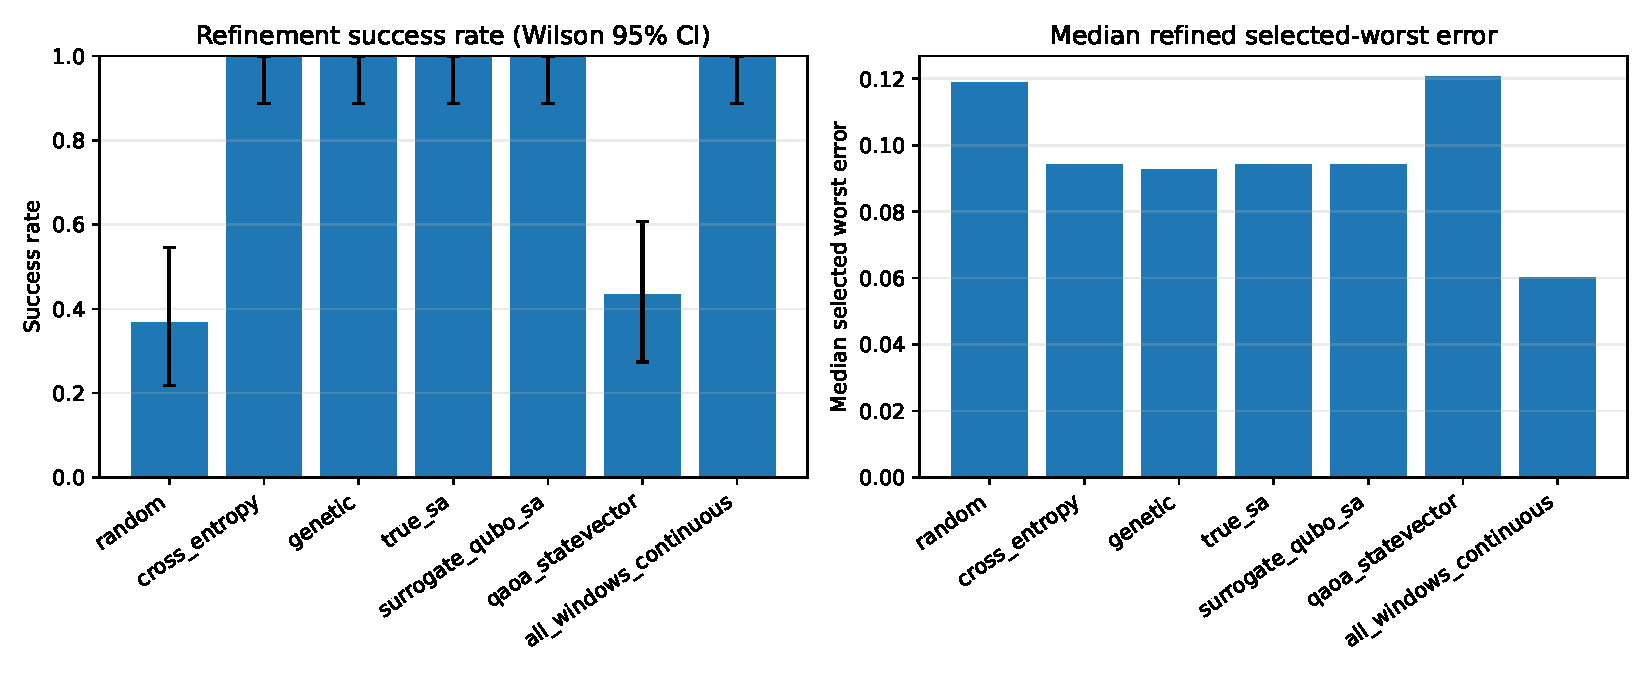
\includegraphics[width=0.72\linewidth]{../figures/phase_shift_cardinality_30seed/main_method_statistics_summary.pdf}
\caption{Thirty-seed main-method statistics for the duty-cycle-prior benchmark. High-duty samplers can be feasible, but all-windows continuous refinement remains lower-error on paired selected-worst comparisons.}
\label{fig:phase_shift_cardinality_30seed}
\end{figure}

\subsection{Focused QAOA/QUBO ablation}

Table~\ref{tab:qaoa_depth_statistics} and Figure~\ref{fig:qaoa_depth_ablation_30seed} isolate the QUBO-sampling step on the same $N=12$ duty-cycle-prior benchmark with 30 deterministic seeds. Each QUBO-derived method uses the same accounting per seed: 96 shared trajectory evaluations to train the QUBO and 24 true post-QUBO candidate evaluations. The resulting raw package contains 150 method--seed rows; the raw method summary table is in the supplement.

The 30-seed success rates with Wilson 95\% intervals are $28/30=0.933$ $[0.787,0.982]$ for surrogate-QUBO simulated annealing, $28/30=0.933$ $[0.787,0.982]$ for exact evaluation of the top 24 QUBO bitstrings, $15/30=0.500$ $[0.332,0.668]$ for random-angle $p=1$ QAOA, $21/30=0.700$ $[0.521,0.833]$ for optimized $p=1$ QAOA, and $29/30=0.967$ $[0.833,0.994]$ for optimized $p=2$ QAOA. Optimized $p=2$ is competitive with the strongest classical QUBO sampler in this narrow statevector QUBO ablation, but it is not statistically supported as superior: versus surrogate-QUBO simulated annealing, its paired success delta is only $+0.033$, the mean selected-worst-error delta is $-0.00056$ with bootstrap 95\% confidence interval $[-0.00393,0.00236]$, and the exact sign-test $p$-value is $0.4545$.

The useful positive result is narrower. Relative to random-angle $p=1$ QAOA, optimized $p=2$ QAOA increases success by $+0.467$ and reduces the mean selected-worst error by $0.0125$ with bootstrap interval $[-0.0188,-0.0060]$. The exact sign-test $p$-value is still not significant at conventional levels ($p=0.2478$), so the evidence should be read as practical improvement in this ablation rather than a formal dominance claim. No quantum advantage is claimed.

\begin{table}[t]
\centering
\caption{Thirty-seed QAOA/QUBO statistical diagnostics. Error deltas are method minus baseline for refined selected-worst error; negative values favor the method.}
\label{tab:qaoa_depth_statistics}
\resizebox{\textwidth}{!}{\begin{tabular}{lllllllll}
\toprule
method & success & wilson\_95\_ci & delta\_success\_vs\_sa & mean\_error\_delta\_vs\_sa & sign\_p\_vs\_sa & delta\_success\_vs\_random\_qaoa & mean\_error\_delta\_vs\_random\_qaoa & sign\_p\_vs\_random\_qaoa \\
\midrule
surrogate\_qubo\_sa & 28/30 & [0.79, 0.98] &  &  &  &  &  &  \\
exact\_qubo\_top24 & 28/30 & [0.79, 0.98] & +0.00 & +0.0006 [-0.0026, +0.0039] & 0.3323 &  &  &  \\
qaoa\_random\_p1 & 15/30 & [0.33, 0.67] & -0.43 & +0.0119 [+0.0053, +0.0184] & 0.5716 &  &  &  \\
qaoa\_optimized\_p1 & 21/30 & [0.52, 0.83] & -0.23 & +0.0048 [-0.0012, +0.0109] & 1.0000 & +0.20 & -0.0072 [-0.0141, -0.0001] & 0.3616 \\
qaoa\_optimized\_p2 & 29/30 & [0.83, 0.99] & +0.03 & -0.0006 [-0.0039, +0.0024] & 0.4545 & +0.47 & -0.0125 [-0.0188, -0.0060] & 0.2478 \\
\bottomrule
\end{tabular}
}
\end{table}

\begin{figure}[t]
\centering
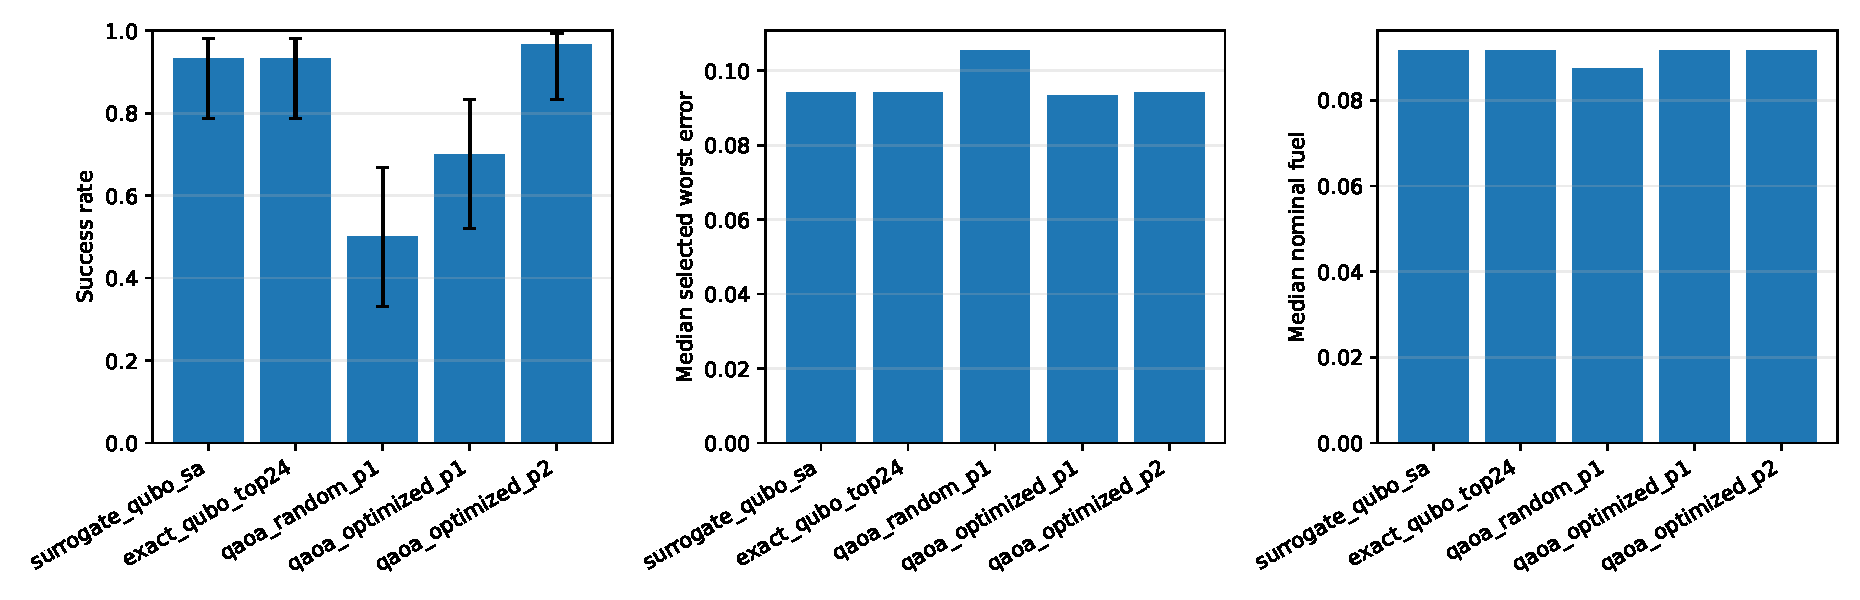
\includegraphics[width=0.72\linewidth]{../figures/qaoa_depth_ablation_30seed/qaoa_depth_ablation_summary.pdf}
\caption{Thirty-seed QAOA-depth ablation summary. Optimized $p=2$ QAOA improves over random-angle QAOA and is competitive with classical QUBO sampling, but paired tests do not support a superiority claim over surrogate-QUBO simulated annealing.}
\label{fig:qaoa_depth_ablation_30seed}
\end{figure}

\subsection{Supplementary diagnostics}

The supplement preserves the evidence that explains how the headline results were reached and where they fail. This includes the original catalog pilot and QUBO fit, feasibility sweeps, direct multiple-shooting and targeted catalog attempts, selected-outage hard-catalog envelope, locked-nominal and delayed-arrival hard-catalog recovery packages, bounded phase-suite and robust-margin rows, direct-collocation and Hermite--Simpson baselines, unrepaired and repaired $N=8$ phase-shift evidence, legacy 10-seed cardinality-prior summaries, cardinality and fuel ablations, and the teacher-controlled benchmark. These artifacts support the failure-mode discussion, but the main claims do not depend on promoting them to primary results.

\section{Discussion}

The central result is a benchmark result, not a sampler-performance claim. Binary thrust-window schedules can be embedded in a reproducible missed-thrust initialization workflow, but the usefulness of a schedule is controlled by the continuous recovery basin. The supplementary diagnostics show both sides: sparse binary schedules can fail even when all-windows continuous refinement succeeds, while duty-cycle priors can preserve enough thrust availability for several samplers to find refinable high-duty schedules.

The 30-seed main-method package is the most relevant initializer evidence. Cross-entropy search, genetic search, true-objective simulated annealing, surrogate-QUBO simulated annealing, and all-windows continuous refinement all succeed in 30/30 seeds on the duty-cycle-prior benchmark, whereas the configured statevector QAOA row succeeds in 13/30 seeds. The paired selected-worst-error tests favor all-windows continuous refinement over every sampled method, and the stricter-threshold sensitivity check shows the sampled high-duty schedules losing pass counts before all-windows continuous does. Thus the paper supports duty-cycle-aware robust initialization as a useful benchmark mechanism, but not a claim that a binary sampler improves the continuous trajectory beyond a strong dense-control baseline.

The focused QAOA/QUBO ablation provides a more favorable but still bounded view of QAOA. Optimizing the angles and increasing simulated depth to $p=2$ improves QAOA relative to random-angle $p=1$ QAOA and is competitive with classical QUBO sampling in that narrow statevector study. The paired comparisons do not support superiority over surrogate-QUBO simulated annealing, and the result is not hardware evidence. For this benchmark, QAOA is best interpreted as a measured initializer family with negative and inconclusive comparisons, not as the contribution itself.

The continuous-backend ladder is useful because it separates what was optimized from what was only diagnosed. The earlier independent-midpoint Hermite--Simpson p=0.4, $a_{\max}=0.2$ row had strong selected-branch and all-mask diagnostic errors, but it optimized only three selected outage branches. The new all-configured headroom package closes that semantic gap for the one-segment phase-shift family: all eight configured masks are optimized and evaluated, with nominal error $0.0111$ and selected/all worst error $0.0774$. Because both rows stop at the configured function-evaluation cap, they are best read as normalized-CR3BP continuous-backend evidence with explicit optimizer-status caveats, not as production collocation parity.

The hard-catalog tail-coast diagnostic addresses a different reviewer concern: whether any hard-catalog missed-thrust recovery case can meet the configured fixed-final-time thresholds once nominal feasibility is locked. The combined one/two-segment row does meet those thresholds, but only within a carefully scoped continuous-backend setup. The final-five-segment coast, locked nominal control, fallback starts, $25/25$ optimizer-converged eligible recovery branches, and two no-recovery-variable late-tail direct evaluations are part of the result. The accepted controls replay exactly under normalized CR3BP but fail the bicircular solar-tidal stress sweep without retuning. A completed fixed-phase retuning batch under the same simple bicircular solar-tidal model also remains negative: at Sun phase $0^\circ$, with the original fixed target and final time and all 27 one/two-segment masks, the retuned nominal error is $0.316772$, configured branch pass count is $19/27$, maximum retuned branch error is $6.0299$, and the strict $(0.05,0.09)$ branch pass count is $16/27$. This narrows a backend blocker and records useful recovery provenance, but it does not establish fuel-optimality, high-fidelity robustness, broader outage-family robustness, or quantum evidence.

The practical implication for astrodynamics researchers is that binary schedule benchmarks should report continuous-backend diagnostics and negative evidence as first-class artifacts. A stronger future initializer claim would need better trajectory-shaped binary encodings, mature continuous optimal-control baselines such as production collocation or sequential convex programming workflows, high-fidelity validation, and statistically significant improvements over strong classical initializers under equal total trajectory-evaluation budgets.

\section{Limitations}

The normalized CR3BP experiments are preliminary-design algorithm studies. They omit ephemeris dynamics, mass depletion, eclipse constraints, navigation uncertainty, thrust pointing limits beyond the acceleration norm, operational constraints, and high-fidelity force modeling. The terminal-error thresholds are screening tolerances; their dimensional interpretation is deliberately large and not comparable to flight targeting requirements.

The continuous backends are research-grade direct shooting, compact direct collocation, Hermite--Simpson, and continuation diagnostics. They are useful for comparing initializer behavior and exposing failure modes, but they are not certified flight-design tools. The new independent-midpoint Hermite--Simpson all-configured row is restricted to the normalized CR3BP one-segment phase-shift family and reaches its configured function-evaluation cap. The recorded-control replay/stress table checks deterministic nominal sidecar replay only. The focused tail-coast accepted-control replay checks persisted branch-control sidecars under normalized CR3BP only; it is not an optimization rerun, high-fidelity validation, production solver parity, fuel-optimal analysis, or quantum evidence. The Horizons ephemeris package is an offline force-model contrast against cached Earth/Moon/Sun geometry, not SPICE validation or ephemeris trajectory replay. The bicircular solar-tidal replay is a simple beyond-CR3BP stress probe and its threshold failures are an external-validity limitation, not SPICE validation. The bicircular retuned recovery package is likewise a simple fixed-phase retuning experiment under the same circular solar-tidal model; even after retuning all configured masks it fails the recorded thresholds and is not SPICE/high-fidelity/flight validation, production solver parity, fuel optimality, or quantum/QUBO/QAOA evidence. The claim evidence ledger clarifies selected-branch, all-mask diagnostic, all-configured-mask, accepted-control replay, force-model-contrast, stress-probe, and retuned-recovery semantics, but it does not add high-fidelity validation. Many supplementary rows optimize selected outage branches and report unselected outage masks diagnostically; only rows that explicitly select all configured masks should be read as all-configured-mask evidence.

The hard-catalog tail-coast result is scoped to a locked-nominal continuous-backend setup with final-five-segment coast, configured one- and two-segment masks, deterministic fallback starts, and late-tail no-recovery-variable direct evaluations. The same controls do not pass the configured bicircular solar-tidal stress sweep, the retuned fixed-phase bicircular batch still fails after retuning, and the cached Horizons contrast shows distance, angular-rate, phase, and solar-tidal acceleration differences not represented by the simple circular stress model. The result therefore does not prove fuel-optimal recovery, high-fidelity robustness, certified flight design, or broader outage-family robustness.

The discrete-initializer conclusions are also bounded. The 30-seed packages improve statistical rigor, but QAOA is simulated with shallow depths and limited optimizer budgets, and the evidence does not support quantum advantage or QAOA superiority. Smaller supplementary packages, including teacher-controlled and legacy 10-seed results, are retained as diagnostics rather than as strong stochastic rankings.

\section{Reproducibility}

The repository contains Python source, configurations, source-state metadata, generated tables, figures, result metadata, cached Horizons query data, and PDFs. The primary artifacts for the main claims are the claim-evidence ledger in \path{data/results/claim_evidence_ledger/}, the independent-midpoint Hermite--Simpson all-configured headroom package in \path{data/results/independent_hs_all_configured_headroom/}, the Horizons ephemeris force-model contrast package in \path{data/results/horizons_ephemeris_force_model_contrast/} with cache \path{data/cache/horizons/hard_catalog_tail_coast_2026jan01_vectors.json}, the bicircular solar-tidal stress package in \path{data/results/bicircular_solar_tidal_stress/}, the completed negative bicircular retuned recovery package in \path{data/results/bicircular_tail_coast_recovery/}, the evidence-synthesis package in \path{data/results/evidence_synthesis/}, the replay/stress sidecar package in \path{data/results/replay_stress_validation/}, the 30-seed main-method package in \path{data/results/phase_shift_cardinality_30seed/}, including the raw-CSV-only threshold-sensitivity artifacts, the 30-seed QAOA/QUBO package in \path{data/results/qaoa_depth_ablation_30seed/}, the hard-catalog tail-coast package in \path{data/results/hard_catalog_tail_coast_recovery/}, and the focused hard-catalog accepted branch-control replay package in \path{data/results/hard_catalog_tail_coast_branch_control_replay/}. The supplement and \path{REPRODUCIBILITY.md} map the secondary diagnostics to their tables, figures, commands, and known caveats.

The reviewer-facing verification path is: start from a clean worktree, rerun the deterministic Horizons ephemeris contrast, bicircular solar-tidal stress, ledger, evidence-synthesis, replay/stress, and accepted branch-control replay postprocessors, rebuild \path{paper/main.pdf} and \path{paper/supplement.pdf} with \texttt{latexmk}, run the smoke tests with Python 3.11, refresh \path{data/results/artifact_manifest.json}, run the manifest checker, and run \texttt{git diff --check}. The completed bicircular retuned recovery artifacts are included in the ledger and manifest, but rerunning that retuning batch is a long evidence-regeneration action rather than a short verification step. Long experiment jobs are not part of the short verification path; recorded artifacts should be used unless evidence is intentionally regenerated.

The manifest is generated by \path{scripts/write_artifact_manifest.py}. Its scoped SHA-256 hashes and byte counts are the authoritative artifact identities. The field \texttt{git\_head\_at\_generation} records the repository state when the manifest was produced; for a committed manifest this necessarily refers to the parent/pre-final state rather than the final commit containing the refreshed manifest. Historical long-run metadata may predate the repository or contain dirty-state records. The current submission snapshot is verified by clean git status after final commit, manifest checking, tests, and local LaTeX builds rather than by interpreting old experiment metadata as final provenance.

\section{Conclusion}

This paper contributes a reproducible normalized CR3BP benchmark resource for robust low-thrust cislunar initialization under missed-thrust events. Its main finding is conservative: duty-cycle-aware binary schedules can help locate refinable high-duty candidates, but all-windows continuous refinement remains lower-error in paired selected-worst comparisons and remains more robust under stricter threshold checks, while the tested simulated QAOA variants do not establish superiority over classical initializers. Deterministic evidence-ledger, evidence-synthesis, sidecar-replay, cached Horizons force-model contrast, and solar-tidal stress layers make the broader validation axes explicit: all-mask continuation, compact collocation, and the new all-configured independent-midpoint Hermite--Simpson package provide phase-shift CR3BP headroom; recorded nominal controls replay consistently; the hard-catalog pass still requires the scoped tail-coast backend; the accepted hard-catalog branch-control sidecars replay exactly under the configured normalized CR3BP model; the cached ephemeris contrast quantifies simple circular force-model omissions; and those same controls fail the configured bicircular solar-tidal stress sweep. A completed simple bicircular retuning batch at fixed Sun phase $0^\circ$ also fails rather than upgrading the result to beyond-CR3BP validation. The useful outcome is therefore an auditable benchmark with negative evidence, failure modes, and provenance, not a claim of quantum advantage or flight-ready robustness.

\section*{Declaration of Competing Interest}
The author declares no known competing financial interests or personal relationships that could have appeared to influence the work reported in this paper.

\section*{Data and Code Availability}
All code and generated artifacts are available in the working repository associated with this draft. The benchmark source states are derived from the NASA/JPL Three-Body Periodic Orbits API and recorded in \path{data/source_states.json}. The Horizons force-model contrast runs offline from the committed cache in \path{data/cache/horizons/}, whose metadata records exact API URLs and query parameters. No archival DOI has been assigned yet; \path{ARCHIVAL_RELEASE.md} keeps the DOI field as TBD until an external repository deposit provides a real identifier.

\bibliographystyle{elsarticle-num}
\bibliography{references}

\end{document}
